\documentclass[letterpaper, 11pt]{article}
\usepackage{latexsym}
\usepackage{amssymb}
\usepackage{times}
\usepackage{graphicx}
\usepackage{amsmath,amsfonts,amsthm}
\usepackage[margin=1in]{geometry}

\newcommand{\vect}[1]{\boldsymbol{\vec #1}}
\newcommand{\rp}[2]{\left[#1,#2\right]}
\renewcommand{\sin}[1]{\operatorname{sin}\left( #1 \right)}
\renewcommand{\cos}[1]{\operatorname{cos}\left( #1 \right)}
\newcommand{\sinsq}[1]{\operatorname{sin}^2\left( #1 \right)}
\newcommand{\cossq}[1]{\operatorname{cos}^2\left( #1 \right)}
\newcommand{\cosinv}[1]{\operatorname{cos}^{-1}\left( #1 \right)}

\begin{document}

\title{600.445 Computer Integrated Surgery \\ Homework \#2 Solutions}
\author{Ravindra Gaddipati, Doran Walsten}
\maketitle

%%%%%%%%%%%%%%%%%%%%%%%%%%%%%%
\pagebreak
\section*{Question 1}
Note, for any term with two skew elements or small displacement elements, we ignored the contribution of that term to the expression.
%%% Part A %%%
\subsection*{A.}
In order to determine $p_{tip}$, we ultimately need to determine $F_{GE} = [R_{GE},p_{GE}]$ which is the transformation from the reference marker coordinate system to the coordinate system of the tip of the pointer.

\begin{align}
    F_{GE} &= F_{BG}^{-1} F_{BD} F_{DE} \\
    &= 
    \begin{bmatrix}
        R_{BG}^{-1} & -R_{BG}^{-1}p_{BG}\\
        0 & 1 
    \end{bmatrix}
    \begin{bmatrix}
        R_{BD} & p_{BD}\\
        0 & 1 
    \end{bmatrix}
    \begin{bmatrix}
        R_{DE} & p_{DE}\\
        0 & 1 
    \end{bmatrix}\\
    &=
    \begin{bmatrix}
        R_{BG}^{-1} & -R_{BG}^{-1}p_{BG}\\
        0 & 1 
    \end{bmatrix}
    \begin{bmatrix}
        R_{BD}R_{DE} & R_{BD}p_{DE} + p_{BD}\\
        0 & 1 
    \end{bmatrix}\\
    &=
    \begin{bmatrix}
        R_{BG}^{-1}R_{BD}R_{DE} & R_{BG}^{-1}R_{BD}p_{DE} + R_{BG}^{-1}p_{BD}-R_{BG}^{-1}p_{BG}\\
        0 & 1 
    \end{bmatrix}\\
\end{align}

From the matrix above, we can determine that $p_{tip} = R_{BG}^{-1}R_{BD}p_{DE} + R_{BG}^{-1}p_{BD}-R_{BG}^{-1}p_{BG}$.
%%% Part B %%%
\subsection*{B.}
This problem requests that we determine the transformation from the CT image to the actual osteotome blade. A similar procedure is performed, this time expanding from the CT frame to the blade.
%Not sure, but we may need to expand here? Not worth it for now.

\begin{align}
	F_{CK} &= F_{GC}^{-1}F_{BG}^{-1}F_{BH}F_{HK} \\
    \begin{bmatrix} R_{CK} & p_{CK} \end{bmatrix} &= \begin{bmatrix} R_{GC}^{-1}R_{BG}^{-1}R_{BH}R_{HK} & R_{GC}^{-1}R_{BG}^{-1}(R_{BH}p_{HK} + p_{BH}) - R_{GC}^{-1}R_{BG}^{-1}p_{BG}-R_{GC}^{-1}p_{GC} \end{bmatrix}
\end{align}

%%% Part C %%%
\subsection*{C.}
Previously, we defined $p_{tip}$ as the translational component of $F_{GE}$. Including error terms in the transformation from the base reference frame, the expression for $F_{GE}$ becomes $$F_{GE} = (\Delta F_{B}F_{BG}\Delta F_{BG})^{-1}(\Delta F_{B}F_{BD}\Delta F_{BD})F_{DE}$$.
When simplified, an expression for $p_{tip}$ can be found.
\begin{align}
    F_{GE} &= \Delta F_{BG}^{-1}F_{BG}^{-1}\Delta F_{B}^{-1}\Delta F_{B}F_{BD}\Delta F_{BD}F_{DE}\\
    &= (F_{BG}^{-1}\Delta F_{BG})^{-1}F_{BD}\Delta F_{BD}F_{DE}\\  \notag
    &= \begin{bmatrix}
        R_{BG}\Delta R_{BG} & R_{BG}\Delta p_{BG} + p_{BG} \\
        0 & 1 \\
    \end{bmatrix}^{-1} \\
    & \qquad \begin{bmatrix}
        R_{BD}\Delta R_{BD}R_{DE} & R_{BD}\Delta R_{BD}p_{DE} + R_{BD}\Delta p_{BD} + p_{BD} \\
        0 & 1 \\
    \end{bmatrix}\\ \notag
    &= \begin{bmatrix}
        \Delta R_{BG}^{-1}R_{BG}^{-1} & -\Delta R_{BG}\Delta p_{BG} - \Delta R_{BG}^{-1}R_{BG}^{-1}p_{BG} \\
        0 & 1 \\
    \end{bmatrix} \\
    & \qquad \begin{bmatrix}
        R_{BD}\Delta R_{BD}R_{DE} & R_{BD}\Delta R_{BD}p_{DE} + R_{BD}\Delta p_{BD} + p_{BD} \\
        0 & 1 \\
    \end{bmatrix}
\end{align}
Expanding out, the following rotation and translation matrices are determined.
\begin{align}
R_{GE}^* &= \Delta R_{BG}^{-1}R_{BG}^{-1}R_{BD}\Delta R_{BD}R_{DE} \\
p_{GE}^* &= (\Delta R_{BG}^{-1}R_{BG}^{-1})(R_{BD}\Delta R_{BD}p_{DE} + R_{BD}\Delta p_{BD} + p_{BD}) -\Delta R_{BG}\Delta p_{BG} - \Delta R_{BG}^{-1}R_{BG}^{-1}p_{BG}
\end{align}
\\
To find $\Delta p_{tip}$, we use the fact that $\Delta p_{tip} = p_{tip}^* - p_{tip}$.
\begin{align}
	\Delta p_{tip} &= (\Delta R_{BG}^{-1}R_{BG}^{-1})(R_{BD}\Delta R_{BD}p_{DE} + R_{BD}\Delta p_{BD} + p_{BD}) \notag \\
    & \qquad -\Delta R_{BG}\Delta p_{BG} - \Delta R_{BG}^{-1}R_{BG}^{-1}p_{BG} - R_{BG}^{-1}R_{BD}p_{DE} + R_{BG}^{-1}p_{BD}-R_{BG}^{-1}p_{BG}  \\
    &= (\Delta R_{BG}^{-1}R_{BG}^{-1}R_{BD}\Delta R_{BD} - R_{BG}^{-1}R_{BD})p_{DE} + (\Delta R_{BG}^{-1} - I)R_{BG}^{-1}p_{BD}  \notag \\
    & \qquad - (\Delta R_{BG}^{-1} - I)R_{BG}^{-1}p_{BG} + \Delta R_{BG}^{-1}R_{BG}^{-1}R_{BD}\Delta p_{BD} - \Delta R_{BG}\Delta p_{BG}  
\end{align}
Here we can see that rotational error also impacts the final location of $p_{tip}$ as the error propagates through the transformations.
%%% Part D %%%
\subsection*{D.}
We linearize the above expression. Terms with two or more errors were removed as  $\Delta x^2 \approx \epsilon^2 \approx 0$ for small errors.
\begin{align}
\Delta p_{tip} & = R_{BG}^{-1}R_{BD}skew(\alpha_{BD})p_{DE} + skew(-\alpha_{BG})R_{BG}^{-1}R_{BD}p_{DE} \notag \\ 
& \qquad + skew(-\alpha_{BG})R_{BG}^{-1}p_{BD} - skew(-\alpha_{BG})R_{BG}^{-1}p_{BG} \notag \\ 
 & \qquad + R_{BG}R_{BD}\epsilon_{BD} - \epsilon_{BG}
\end{align}
%%% Part E %%%
\subsection*{E.}
Here, we incorporate error into the transformation from the CT frame to the blade frame. 
\begin{align}
	F_{CK}^* &= (F_{GC}\Delta F_{GC})^{-1}(\Delta F_BF_{BG}\Delta F_{BG})^{-1}\Delta F_BF_{BH}\Delta F_{BH}F_{HK} \notag \\
    &= \Delta F_{GC}^{-1}F_{GC}^{-1}\Delta F_{BG}^{-1}F_{BG}^{-1}\Delta F_B^{-1}\Delta F_BF_{BH}\Delta F_{BH}F_{HK} \notag \\
    &= \Delta F_{GC}^{-1}F_{GC}^{-1}\Delta F_{BG}^{-1}F_{BG}^{-1}F_{BH}\Delta F_{BH}F_{HK} \notag
\end{align}
Following simplification, the following expressions can be determined for $R_{CK}^*$ and $p_{CK}^*$.
\begin{align}
	R_{CK}^* &= \Delta R_{GC}^{-1}R_{GC}^{-1}\Delta R_{BG}^{-1}R_{BG}^{-1}R_{BH}\Delta R_{BH}R_{HK} \\
    p_{CK}^* &= \Delta R_{GC}^{-1}R_{GC}^{-1}(\Delta R_{BG}^{-1}R_{BG}^{-1}(R_{BH}\Delta R_{BH}p_{HK} + R_{BH}\Delta p_{BH} + p_{BH}) \notag \\ 
    & \qquad - \Delta R_{BG}^{-1}\Delta p_{BG} - \Delta R_{BG}^{-1}R_{BG}^{-1}p_{BG}) - \Delta R_{GC}^{-1}\Delta p_{GC} - \Delta R_{GC}^{-1}R_{GC}^{-1}p_{GC}
\end{align}

As done in part C, we will use $\Delta R_{CK} = R_{CK}^* - R_{CK}$ and $\Delta p_{CK} = p_{CK}^* - p_{CK}$.

\begin{align}
	\Delta R_{CK} &= \Delta R_{GC}^{-1}R_{GC}^{-1}\Delta R_{BG}^{-1}R_{BG}^{-1}R_{BH}\Delta R_{BH}R_{HK} - R_{GC}^{-1}R_{BG}^{-1}R_{BH}R_{HK} \\
    \Delta p_{CK} &= \Delta R_{GC}^{-1}R_{GC}^{-1}(\Delta R_{BG}^{-1}R_{BG}^{-1}(R_{BH}\Delta R_{BH}p_{HK} + R_{BH}\Delta p_{BH} + p_{BH}) \notag \\ 
    & \qquad \qquad \qquad \quad -\Delta R_{BG}^{-1}\Delta p_{BG} - \Delta R_{BG}^{-1}R_{BG}^{-1}p_{BG}) \notag \\
	& \qquad - R_{GC}^{-1}R_{BG}^{-1}(R_{BH}p_{HK} + p_{BH}) - R_{GC}^{-1}R_{BG}^{-1}p_{BG}-R_{GC}^{-1}p_{GC} \\
   	&= (\Delta R_{GC}^{-1}R_{GC}^{-1}\Delta R_{BG}^{-1}R_{BG}^{-1}R_{BH}\Delta R_{BH} - R_{GC}^{-1}R_{BG}^{-1}R_{BH})p_{HK} \notag \\
   	& \qquad + (\Delta R_{GC}^{-1}R_{GC}^{-1}\Delta R_{BG}^{-1}R_{BG}^{-1} - R_{GC}^{-1}R_{BG}^{-1})(p_{BH} - p_{BG}) \notag \\ 
    & \qquad + \Delta R_{GC}^{-1}R_{GC}^{-1}\Delta R_{BG}^{-1}R_{BG}^{-1}R_{BH}\Delta p_{BH} \notag \\
    & \qquad - \Delta R_{GC}^{-1}R_{GC}^{-1}\Delta R_{BG}^{-1}\Delta p_{BG} - (\Delta R_{GC}^{-1} - I)R_{GC}^{-1}p_{GC} - \Delta R_{GC}^{-1}\Delta p_{GC}
\end{align}
%%% Part F %%%
\subsection*{F.}
Next, we linearized the expressions above.
\begin{align}
	\Delta R_{CK} &= (I + skew(-\alpha_{GC}))R_{GC}^{-1}(I + skew(-\alpha_{BG}))R_{BG}^{-1}R_{BH}(I +skew(\alpha_{BH}))R_{HK} \notag \\ 
    & \qquad - R_{GC}^{-1}R_{BG}^{-1}R_{BH}R_{HK} \\
    &= (R_{GC}^{-1} + skew(-\alpha_{GC})R_{GC}^{-1})(R_{BG}^{-1} + skew(-\alpha_{BG})R_{BG}^{-1}) \notag \\ 
    & \qquad * (R_{BH}R_{HK} + R_{BH}skew(\alpha_{BH})R_{HK}) - R_{GC}^{-1}R_{BG}^{-1}R_{BH}R_{HK} \\
    &= (R_{GC}^{-1}R_{BG}^{-1} + R_{GC}^{-1}skew(-\alpha_{BG})R_{BG}^{-1} + skew(-\alpha_{GC})R_{GC}^{-1}R_{BG}^{-1}) \notag \\ 
    & \qquad * (R_{BH}R_{HK} + R_{BH}skew(\alpha_{BH})R_{HK}) -R_{GC}^{-1}R_{BG}^{-1}R_{BH}R_{HK} \\
    &= R_{GC}^{-1}R_{BG}^{-1}R_{BH}R_{HK} + R_{GC}^{-1}R_{BG}^{-1}R_{BH}skew(\alpha_{BH})R_{HK} + R_{GC}^{-1}skew(-\alpha_{BG})R_{BG}^{-1}R_{BH}R_{HK}  \notag \\ 
    & \qquad + skew(-\alpha_{GC})R_{GC}^{-1}R_{BG}^{-1}R_{BH}R_{HK} -  R_{GC}^{-1}R_{BG}^{-1}R_{BH}R_{HK} \\
    &= R_{GC}^{-1}R_{BG}^{-1}R_{BH}skew(\alpha_{BH})R_{HK} + R_{GC}^{-1}skew(-\alpha_{BG})R_{BG}^{-1}R_{BH}R_{HK} \notag \\
    & \qquad + skew(-\alpha_{GC})R_{GC}^{-1}R_{BG}^{-1}R_{BH}R_{HK} \\
	\Delta p_{CK} &= (R_{GC}^{-1}R_{BG}^{-1}R_{BH}skew(\alpha_{BH}) + R_{GC}^{-1}skew(-\alpha_{BG})R_{BG}^{-1}R_{BH} + skew(\alpha_{GC})R_{GC}^{-1}R_{BG}^{-1}R_{BH})p_{HK}  \notag \\ 
    & \qquad  +  (R_{GC}^{-1}skew(-\alpha_{BG})R_{BG}^{-1} + skew(-\alpha_{GC})R_{GC}^{-1}R_{BG}^{-1})(p_{BH} - p_{BG})  \notag \\ 
    & \qquad  + (R_{GC}^{-1}R_{BG}^{-1} + R_{GC}^{-1}skew(-\alpha_{BG})R_{BG}^{-1} + skew(-\alpha_{GC})R_{GC}^{-1}R_{BG}^{-1})R_{BH}\epsilon_{BH} \notag \\ 
    & \qquad  - (R_{GC}^{-1} + skew(-\alpha_{GC})R_{GC}^{-1} + R_{GC}^{-1}skew(-\alpha_{BG}))\epsilon_{BG} \notag \\ 
    & \qquad  - skew(-\alpha_{GC})R_{GC}^{-1}p_{GC} - \epsilon_{GC}
\end{align}

%%% Part G %%%
\subsection*{G.}
As in previous sections, we assume that any terms developed during linearization that contain 2+ skew and/or epsilon terms are ignored.

We begin by defining the relationship between $F_{GC}^* = F_{GC}\Delta F_{GC}$ and $b_k^* = b_k + \Delta  b_k$ then simplify.

\begin{align}
	b_k^* &= F_{GC}\Delta F_{GC}a_{k} \\
    &= \begin{bmatrix}
    	R_{GC} & p_{GC} \\
        0 & 1
    \end{bmatrix}
    \begin{bmatrix}
    	\Delta R_{GC} & \Delta p_{GC} \\
        0 & 1 
    \end{bmatrix}
    \begin{bmatrix}
    a_k \\
    1
    \end{bmatrix} \\ 
    &= \begin{bmatrix}
    	R_{GC} & p_{GC} \\
        0 & 1
    \end{bmatrix}
    \begin{bmatrix}
    	\Delta R_{GC}a_k + \Delta p_{GC} \\
        1 
    \end{bmatrix} \\
    &= R_{GC}\Delta R_{GC}a_k + R_{GC}\Delta p_{GC} + p_{GC} \\
    &= R_{GC}(I + skew(\alpha_{GC}))a_k + R_{GC}\epsilon_{GC} + p_{GC} \\ 
    b_k + \Delta b_k &= R_{GC}a_k + p_{GC} + R_{GC}skew(\alpha_{GC})a_k + R_{GC}\epsilon_{GC} \\
    \Delta b_k &= R_{GC}skew(\alpha_{GC})a_k + R_{GC}\epsilon_{GC} \\
    &= R_{GC}(\alpha_{GC} \times a_k + \epsilon_{GC}) \\
    &= R_{GC}(-a_k \times \alpha_{GC} + \epsilon_{GC}) \\
    &= R_{GC}(skew(-a_k)\alpha_{GC} + \epsilon_{GC}) \\ 
     \Delta b_k &= \begin{bmatrix}
    	R_{GC} & R_{GC}skew(-a_k)
    \end{bmatrix} 
    \begin{bmatrix}
    	\epsilon_{GC} \\
        \alpha_{GC}
     \end{bmatrix} \\
\end{align}

Given the constraint function $f$, we can put a bound on the matrix product evaluated above.
$$0 \leq f\left(\begin{bmatrix}
    	R_{GC} & R_{GC}skew(-a_k)
    \end{bmatrix} 
    \begin{bmatrix}
    	\epsilon_{GC} \\
        \alpha_{GC}
     \end{bmatrix}\right) \leq \eta_k$$
Both the rotational and transnational components of the error are bounded by $\eta_k$. This error comes entirely from registration.
%%% Part H %%%
\subsection*{H.}
In this section, we add segmentation error into the previous problem as $a_k^* = a_k + \Delta a_k$. Using the matrix algebra above with the adjusted $a_k^*$ term:

\begin{align}
	b_k^* &= R_{GC}\Delta R_{GC}a_k + R_{GC}\Delta R_{GC}\Delta a_k + R_{GC}\Delta p_{GC} + p_{GC} \\
    &= R_{GC}(I + skew(\alpha_{GC})a_k + R_{GC}(I + skew(\alpha_{GC}))\Delta a_k + R_{GC}\epsilon_{GC} + p_{GC} \\
    b_k + \Delta b_k &= R_{GC}a_k + p_{GC} + R_{GC}skew(\alpha_{GC})a_k + R_{GC}\Delta a_k + R_{GC}skew(\alpha_{GC})\Delta a_k + R_{GC}\epsilon_{GC} \\
    &= R_{GC}(\alpha_{GC} \times a_k +\Delta a_k + \epsilon_{GC})  \\
    &= R_{GC}(-a_k \times \alpha_{GC} + \Delta a_k + \epsilon_{GC}) \\
    &= R_{GC}(skew(-a_k)\alpha_{GC} + \Delta a_k + \epsilon_{GC}) \\
    \Delta b_k &= \begin{bmatrix}
    	R_{GC} & R_{GC} & R_{GC}skew(-a_k)
    \end{bmatrix}
    \begin{bmatrix}
    	\Delta a_k \\
        \epsilon_{GC} \\
        \alpha_{GC}
    \end{bmatrix}
\end{align}

Given the two constraint function on both $\Delta b_k$ and $\Delta a_k$, we can define a global constraint function which considers both constraints:

$$ 0 \leq f\left(\begin{bmatrix} 
			R_{GC} & R_{GC} & R_{GC}skew(-a_k) \\
            I & 0 & 0
          \end{bmatrix}
          \begin{bmatrix}
    		\Delta a_k \\
        	\epsilon_{GC} \\
        	\alpha_{GC}
    	  \end{bmatrix}\right) \leq \begin{bmatrix}
          						\eta_k \\
                                \xi_k
                              \end{bmatrix} $$
%%%%%%%%%%%%%%%%%%%%%%%%%%%%%%

\section*{Question 2}
%%% Part A %%%
\subsection*{A.}

We're assuming plate coordinates is the CT coordinates. In this problem, we are trying to find where to drill the holes $g_k$ in the CT frame given that we know what the plate looks like with the desired acetabular component transformation $F_{CA}$.

$$g_k=F^{-1}_{CA}q_k$$

%%% Part B %%%
\subsection*{B.}
In part 1H, we bounded the error of $F_{GC}$ in the real world. Since we are planning the holes in the CT frame, this bound influences how accurately we must place the holes in the CT space. If we want our tracking error ($\Delta \vec{b}_k$) to be bounded by $\eta_k$, then the error inherent within our registration transformation must be bounded as follows, where $f$ is our constraint function:
$$ 0 \leq f\left(\begin{bmatrix} 
			R_{GC} & R_{GC} & R_{GC}skew(-a_k) \\
            I & 0 & 0
          \end{bmatrix}
          \begin{bmatrix}
    		\Delta a_k \\
        	\epsilon_{GC} \\
        	\alpha_{GC}
    	  \end{bmatrix}\right) \leq \begin{bmatrix}
          						\eta_k \\
                                \xi_k
                              \end{bmatrix} $$

%%% Part C %%%
\subsection*{C.}
As suggested on the homework assignment, let us represent the transformation between the plate and the rest of the pelvis by $F_{PC}$ and the transformation between the acetabular component of the pelvis and plate by $F_{AP}$. We can then define the transformation from the pelvis to the acetabular component $F_{CA}$ as:
$$F_{CA} = F_{PC}^{-1}F_{AP}^{-1}$$

We can incorporate error due to misalignment by including error terms:

$$F_{CA}\Delta F_{CA} = \Delta F_{PC}^{-1}F_{PC}^{-1}\Delta F_{AP}^{-1}F_{AP}^{-1}$$

At each of the junctions of the plate and the bone fragments, there can be translational and rotational error caused by movement of the plate around the holes. The worst cases are shown below:  \begin{center}
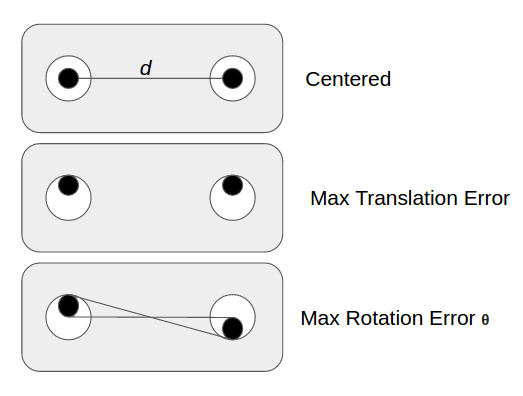
\includegraphics[scale=0.4]{hole_error.png}
\end{center}

Though both rotation error and translation error are constrained to each other by the geometry of the holes, we assume they are independent and consider an upper bound to error. As such we assume maximum translational error of $\rho/2$ if the plate slides one direction completely, and a max rotational error of $\rho/d$ where $d$ is the distance between the two holes. Since these are small distances, we use the small angle approximation. This can be represented as

$$\Delta R = I - skew(\alpha_{\rho/d})$$
$$\Delta p = \frac{\rho}{2}$$

Inserting these expressions within the error transformations allows us to evaluate an expression for $\Delta F_{CA}$.

\begin{align*}
	F_{CA}\Delta F_{CA} &= \begin{bmatrix}
    						R_{PC}\Delta R & R_{PC}\Delta p + p_{PC} \\
                            0 & 1
                          \end{bmatrix}^{-1} 
                          \begin{bmatrix}
                          	R_{AP}\Delta R & R_{AP}\Delta p + p_{AP}\\
                            0 & 1
                          \end{bmatrix}^{-1}\\
   &= \begin{bmatrix}
       \Delta R^{-1}R_{PC}^{-1} & - \Delta R^{-1}\Delta p -\Delta R^{-1}R_{PC}^{-1}p_{PC}\\
       0 & 1
       \end{bmatrix}
       \begin{bmatrix}
      \Delta R^{-1}R_{AP}^{-1} & -\Delta R^{-1}\Delta p -\Delta R^{-1}R_{AP}^{-1}p_{AP}\\
       0 & 1
       \end{bmatrix} \\
 &= \begin{bmatrix}
 		\Delta R^{-1}R_{PC}^{-1}\Delta R^{-1}R_{AP}^{-1} & \Delta R^{-1}R_{PC}^{-1}(-\Delta R^{-1}\Delta p -\Delta R^{-1}R_{AP}^{-1}p_{AP}) -\Delta R^{-1}\Delta p \\ 
        &-\Delta R^{-1}R_{PC}^{-1}p_{PC}
    \end{bmatrix}
\end{align*}

When this matrix is linearized and the ideal rotation and translation are removed from the remaining terms, we determine the rotational and translational error of the entire transformation. (Note: We eliminated any terms with 2+ skew and/or minute displacement terms).

$$\Delta R_{CA} = R_{PC}^{-1}skew(-\alpha_{\rho/d})R_{AP}^{-1} + skew(-\alpha_{\rho/d})R_{PC}^{-1}R_{AP}^{-1}$$
$$\Delta p_{CA} = -skew(-\alpha_{\rho/d})R_{PC}^{-1}p_{PC} - (R_{PC}^{-1}skew(-\alpha_{\rho/d})R_{AP}^{-1} + skew(-\alpha_{\rho/d})R_{PC}^{-1}R_{AP}^{-1})p_{AP} - R_{PC}^{-1}\frac{\rho}{2} - \frac{\rho}{2}$$


%%%%%%%%%%%%%%%%%%%%%%%%%%%%%%
\section*{Question 3}
%%% Part A %%%
\subsection*{A.}
For simplicity in calculation, we will assume that the tracking system is accurate as we as our registration transformation. Since we have two cannulated pins placed in the pelvis, each registration point is able to to lock two angles as well as a 3D point in space. Using the two pins gives us enough constraints to solve the system. The challenge posed by this system is determining how to relate these two different pieces of information together to allow us to register the system.

Here is a high-level summary of the steps the surgeon will complete to collect the data required for us to make the registration transformation:

\begin{enumerate}
\item The surgeon will push the pointer to the bottom of the first cannula. This conformation will be represented as $v_1$.
\item The surgeon will then raise the pointer to a 2nd point still within the first cannula. The vector created by the difference of this position with $v_1$ in the $F_G$ reference frame will be represented as $a_1$.
\item The surgeon will repeat Step 1 and Step 2 for the second cannula, generating $v_2$ and $a_2$ respectively.
\item We then compute the registration transformation $F_{GC}$ using these parameters.
\end{enumerate}

The steps to complete the registration step are as follows:
\begin{enumerate}
\item Use a phantom midpoint in both the $F_G$ and $F_{C}$ reference frames to generate two vector-point pairs used to approximate $R_{GC}$
\item Normalize the "rotation" matrix $R_{GC}$ so it actually is a rotation matrix and determine the 3 rotation angles which define the rotation
\item Minimize the cross product of the registered cannula axes in the CT frame to the calculated axes $a_x$ in the real world $F_G$ frame in order to ensure the axes are parallel
\item Use the rotation matrix $R_{GC}$ to solve for the registration translation $p_{GC}$.
\end{enumerate}

The theory behind this approach is that we are unable to generate 3 points from which to perform a tradition least-squares estimation of the registration rotation $R_{GC}$. We account for this by generating the best estimate for this rotation from the two points provided. We have the additional information that the axes of the pointer and cannula are parallel. This means that the cross product of the axes should be minimized (in theory, \textbf{0}) when registered to the proper reference frame. In this case, we register the axes of each cannula in the CT frame to the marker $F_G$ frame then minimize the cross product of each with the corresponding axes in the $F_{G}$ simultaneously. This can be done through gradient descent over variables which define the registration rotation $R_{GC}$. 
\\
\\
A summary of the relevant equations in this computation is below.

\subsection*{Vector Pairs}
When the surgeon generates $v_1$, the mathematical relationship between the frames is as follows:
\begin{align}
	v_1 &= F_{GC}F_{Ck,1} \notag \\
    &= F_{GC}p_{Ck,1} \tag{Location of pin base in CT} \\
    &= R_{GC}p_{Ck,1} + p_{GC} \notag
\end{align}

The same can be repeated for $v_2$ in the second cannula. We generate a phantom point in both the CT frame $F_{C}$ and the marker frame $F_{G}$ by taking the midpoint of $p_{Ck,1}$,$p_{Ck,2}$ and $v_1$,$v_2$. We will call these points $v_m$ and $p_{Ck,m}$, respectively. We can then define the following vectors between the midpoint and the original points.
$$b_1 = v_1 - v_m$$
$$b_2 = v_2 - v_m$$
$$c_1 = p_{Ck,1} - p_{Ck,m}$$
$$c_2 = p_{Ck,2} - p_{Ck,m}$$

We can use the registration transformation to solve for $R_{GC}$
\begin{align}
	F_{GC}c_1 &= R_{GC}c_1 + p_{GC} \\
    R_{GC}c_1 + p_{GC} &= R_{GC}(p_{Ck,1} - p_{Ck,m}) - p_{GC} \\
    R_{GC}c_1 &= R_{GC}p_{Ck,1} + p_{GC} - R_{GC}p_{Ck,m} - p_{GC} \\
    &= v_1 - v_m \\
    &= b_1
\end{align}

This process can be repeated for $c_2$ as well. This generates the system of equations:
$$R_{GC}C = B$$
Where $C = [c_1, c_2]$, $B = [b_1, b_2]$. We can thus approximate $R_{GC}$ as $R_{GC} = BPinv(C)$, where $Pinv$ represents the pseudoinverse of C.

\subsection*{Renormalize $R_{GC}$}
Using the normalization technique suggested in the lecture slides, we can build an estimated rotation matrix $R_{GC}$. Before moving onto the next step, we will determine the yaw, pitch, and roll ($\alpha$,$\beta$,$\gamma$) of this estimated matrix.

\subsection*{Minimize Cross Product}
The z-axis of the first cannula can be represented as $R_{Ck,1}[0,0,1]^T + p_{Ck,1}$ in CT frame coordinates. When this axis is registered to the marker frame, the new expression is $R_{GC}R_{Ck,1}[0,0,1]^T + R_{GC}p_{Ck,1} + p_{GC}$. From our earlier analysis, we determined $R_{GC}p_{Ck,1} + p_{GC} = v_1$, thus our expression for the z-axis of the cannula in marker frame coordinates is $R_{GC}R_{Ck,1}[0,0,1]^T + v_1$.

We are told in the problem that the axes of the cannula and pointer align. This means that the cross product of vectors parallel to this axis will be zero. We computed such a vector $a_1$ during the initial setup. Thus, it is our goal to select $R_{GC}$ that solves the minimization problem below
\begin{align}
\min_{R_{GC}} \|skew(a_1)(R_{GC}p_{Ck,1} + v_1)\|^2
\end{align}
However, we have the benefit of a second equation to minimize simultaneously as there are two cannulas from which we computed axes in the marker space. In that case, we would take the cross product of the computed $a_2$ vector with the registered axis of the second cannula in the CT frame. After completing the same math above, the resultant minimization problem is:
\begin{align}
\min_{\alpha,\beta,\gamma} \|skew(a_1)(R_{GC}(\alpha,\beta,\gamma)p_{Ck,1} + v_1)\|^2 + \|skew(a_2)(R_{GC}(\alpha,\beta,\gamma)p_{Ck,2} + v_2)\|^2
\end{align}
In the previous step, we determined the initial estimates of yaw, pitch, and roll ($\alpha,\beta,\gamma$) of the matrix $R_{GC}$. We can use a gradient descent approach on these three parameters to solve the minimization problem above for the optimal yaw, pitch, and roll. Our hope is that by providing an initial estimate of the rotation based on the existing 3D points, the gradient descent will find a solution that is closest to the rotation matrix required. If no initial estimate had been provided, there is a risk that the gradient descent would find an alternative solution to the minimization problem which does does not satisfy the previous equation for the vector pairs.

\subsection*{Estimate Displacement}
Finally, we use the computed rotation matrix $R_{GC}$ to estimate the translation $p_{GC}$. This estimation can be completed using the phantom midpoints created previously: $p_{GC} = v_m - R_{GC}p_{Ck,m}$. 

As mentioned in the problem description, we cannot guarantee that the surgeon pushes the tip of the pointer to the bottom of the cannula. So we introduce this as an error term in $v_1$ and $v_2$. 
\begin{align}
v_1 &= F_{BG}^{-1}F_{BD,1}F_{DE}\Delta b_1 \\
v_2 &= F_{BG}^{-1}F_{BD,2}F_{DE}\Delta b_2
\end{align}
Depending on the design of the cannulas, we can bound these errors by a reasonable value during calculation of the registration transformation.

\subsection*{Discussion}
There are certainly limitations to the method above. We currently only include one source of error (pointer depth) and were uncertain how to best integrate the axes information with the necessary position information to determine where along the aligned axes the pointer lies.
\subsubsection*{Method 2}
The known transformations from $F_C$ to each cannula are enough to fully constrain the system (unless the two are in the same plane), but we were unsure how to effectively use that information. A method we explored was equating the transformation from $F_C$ to the pins with the transformation from $F_G$ to $p_tip + p_z$, where $p_z$ is a displacement in the Z axis of the pin frame. However we were unable to fully solve the system of equations.

  
%%% Part B %%%
\subsection*{B.}
Since the probe is damaged, we can no longer assume the probe axis is inline with the cannula axis. In this method of registration, the surgeon inserts the probe into the cannula, and collects multiple points by rotating the probe within the cannula. By rotating the probe, we can measure the angular offset of the probe using the consistent depth. This method has the advantage that it can be used regardless of a damaged shaft- it could also be used to verify the probe is not damaged.
\begin{center}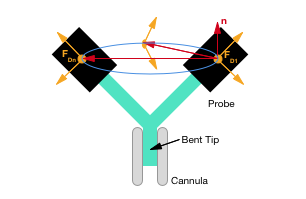
\includegraphics[scale=1]{Circle_in_Space.png}\end{center}
Let $P_{exp}$ be the portion of the probe above the bend, and $P_t$ be the zero-error location of the tip in the $F_D$ frame. As the probe rotates, the collected points will be in the same plane, and a set of vectors $v_1,...,v_n$.  We compute the cross product and normalize, obtaining the axis of the probe tip, as well as the radius of the circle. Using the system of transformations from each point to the norm, we compute $R_{circle}$. The final location of the probe tip in the $F_D$ frame is given by
\begin{align}
\vect p_{tip} = \vect p_{exp} + R_{circle}^{-1}(\vect p_t - \vect p_{exp})
\end{align}
Where $R_{circle}$ is solved from the system of equations then normalized to become a true rotation
\begin{align}
R_{circle}
\begin{bmatrix}
F_{BG}^{-1}F_{BD_1} \begin{bmatrix} 0 \\ 0 \\ 1 \\ 1 \end{bmatrix}
& ... &
F_{BG}^{-1}F_{BD_n} \begin{bmatrix} 0 \\ 0 \\ 1 \\ 1 \end{bmatrix}
\end{bmatrix}
= \begin{bmatrix}
\vect n_1 & ... & \vect n_n
\end{bmatrix}
\end{align}
Let $\vect v_i = p_x - p_y$ for the measurements $x,y$ along the circle in the $F_G$ frame. $\vect n_i$ is computed from each vector pair:
\begin{align}
\vect n_i = \frac{\vect v_i \times \vect v_j}{||\vect v_i \times \vect v_j ||}
\end{align}
$\vect p_{exp}$ becomes
\begin{align}
\vect p_{exp} = \frac{\vect p_t}{||p_t||}\cdot\left(\frac{||r||}{\sin{\theta}}\right)
\end{align}
$\theta$ represents the angle of our bend, and $P_t = P_{tip}$ if there is no error, and the expected $F_{DE}$ is true. We transform $\vect n_i$ into the $F_D$ frame from the $F_G$ frame, and compute theta using the dot product of the normalized vectors
\begin{align}
\theta = \cosinv{F_{BD}^{-1}F_{BG}\vect n_i \cdot\begin{bmatrix} 0 \\ 0 \\ 1 \end{bmatrix}}
\end{align}
The axis of the pins is given by $\vect n_i$ centered on the origin of the fitted circle. We may compute the average to obtain the most representative vector. 

To determine the corrected $F_DE$, we use the rotation to the norm of the circle computer earlier, $R_{circle}$ as $R_{DE}$. The new displacement can be expressed as the sum of the exposed section of the probe computed in (59) and the rotated bent tip. To compute this bend, we compute the difference of $P_t$ and $P_exp$, transform it from the $F_D$ frame to the $F_G$ frame to rotate it, then transform it back to the $F_D$ frame. This method gives us the true $p_{tip}$.
\begin{align}
F_{DE} = [R_{circle}, \vect p_{exp} + F_{BD}^{-1} F_{BG}R_{circle}^{-1} F_{BG}^{-1}F_{BD}(P_t - P_{exp})]
\end{align}


%%%%%%%%%%%%%%%%%%%%%%%%%%%%%%
\section*{Question 4}
A unit quaternion $q=\rp{\cos{\frac{\theta}{2}}}{\sin{\frac{\theta}{2}}\vect{n}}$ can be used to represent a rotation by an angle $\theta$ about an axis $\vect n$ where $\vect n$ is a unit vector. Provide a proof, i.e. demonstrate that for arbitrary $\vect p$:
$$\rp{0}{\mathrm{Rot}(\vect n, \theta) \cdot \vect p}=\rp{\cos{\frac{\theta}{2}}}{\sin{\frac{\theta}{2}}\vect n} \circ \rp{0}{\vect p} \circ \rp{\cos{\frac{\theta}{2}}}{-\sin{\frac{\theta}{2}}\vect n}$$
Let $\vect v$ be the quaternion rotation. Evaluating the product and simplifying, we obtain:
\begin{align}
\vect v &= \rp{-\sin{\theta/2} \vect n \cdot \vect p}{\cos{\theta/2} \vect p + \sin{\theta/2} \times \vect p} \rp{\cos{\theta/2}}{-\sin{\theta/2}\vect n} \\
&= [-\sin{\theta/2}\vect n \vect p \cos{\theta/2}(\cos{\theta/2}\vect p  + \sin{\theta/2}\vect n \times \vect p)(-\sin{\theta/2})\vect n,\notag \\ 
    & \qquad (-\sin{\theta/2}\vect n \vect p)(-\sin{\theta/2}\vect n) + (\cos{\theta/2})(\cos{\theta/2}\vect p + \sin{\theta/2} \vect n \times \vect p) \notag \\ 
    & \qquad + (\cos{\theta/2}\vect p + \sin{\theta/2}\vect n \times \vect p)\times (-\sin{\theta/2}\vect n)] \\
    &= [0,-\sinsq{\theta/2}\vect n \vect p \vect n + \cos{\theta/2} \vect p + \notag \\ 
    & \qquad \cos{\theta/2}\sin{\theta/2}\vect n \times \vect p + (-\sin{\theta/2}\vect n)\times(\cos{\theta/2}\vect n)] \\
    &= [0, -\sinsq{\theta/2} \vect n \vect p \vect n + \cossq{\theta/2}\vect p + 2(\vect n \times \vect p)\cos{\theta/2}\sin{\theta/2}] \\
    &= [0, \vect p \cos{\theta} + (\vect n \times \vect p) \sin{\theta} + n(n \cdot p)(1- \cos{\theta})]
\end{align}
Here we made use of dot and cross product properties, as well has the half angle identity. Evaluating the quaternion rotation yields the Rodrigues rotation formula for a rotation angle $\theta$ of $\vect v$ about unit vector $\vect k$ :
\begin{align}
Rot[\vect k, \theta] \cdot \vect v = \vect v \cos{\theta} + (\vect k \times \vect v) \sin{\theta} + \vect k(\vect k \cdot \vect v)(1-\cos{\theta})
\end{align}
Thus, we can say that the quaternion can be used to represent a rotation of an arbitrary vector $\vect p$ about the unit vector $\vect n$:
\begin{align}
\vect v &= [0, \vect p \cos{\theta} + (\vect n \times \vect p) \sin{\theta} + \vect n(\vect n \cdot \vect p)(1- \cos{\theta})] \\
&= \rp{0}{Rot(\vect n, \theta) \cdot \vect p}
\end{align}

\end{document}
